\documentclass{book}
\usepackage[landscape,a3paper,left=0.5cm,right=1in,top=1in,bottom=1in]{geometry}
\usepackage{amsmath}
\usepackage{xcolor}
\usepackage{tikz}
\usepackage{pgfplots}
\usepackage{booktabs}
\usepackage{multirow}
\usepackage{amsmath,amssymb}

\begin{document}

\vspace{2cm}

\begin{figure}\caption{\textsc{Equiv + Permut} for Test of 93 small instances of netlib}
\vspace{0.5cm}\centering

\begin{tabular}{ccc} & gecode & coinbc\\\\\tikz{\node (a) at (0.0,2.5) {\textsc{QuadraMod}};\node (a) at (0.0,0) {};} & 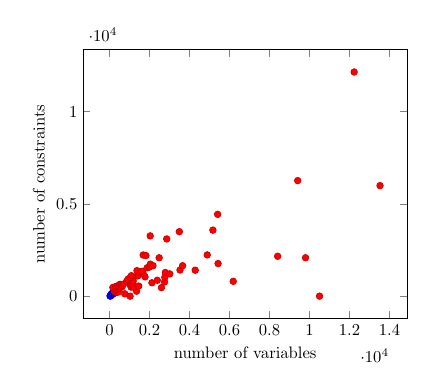
\begin{tikzpicture}[scale=0.6]
\begin{axis}[scatter, point meta=\thisrow{time}, only marks, colorbar, colorbar horizontal,colorbar style={ylabel={Time (min)}, ylabel style={rotate=270},}, colorbar to name={storedcolorbar1},, xlabel=number of variables,ylabel=number of constraints]

\addplot table[x=x,y=y]  { 
 x y time
 33 34 0.05 
 33 34 0.0 
 42 60 0.0 
 49 71 0.0 
 98 68 0.0 
 80 107 0.0 
 84 116 0.0 
 104 151 2.0 
 112 165 1.0 
 143 164 2.0 
 141 180 2.0 
 1027 26 2880.0 
 181 159 3.0 
 163 185 2.0 
 226 197 13.0 
 204 250 6.0 
 283 206 13.0 
 204 295 23.0 
 263 264 2880.0 
 309 242 2880.0 
 250 305 2880.0 
 164 495 2880.0 
 302 281 2880.0 
 423 246 2880.0 
 761 155 2880.0 
 316 381 2880.0 
 354 404 2880.0 
 303 545 2880.0 
 481 421 2880.0 
 359 565 2880.0 
 474 446 2880.0 
 458 469 2880.0 
 473 539 2880.0 
 468 566 2880.0 
 10501 27 2880.0 
 615 522 2880.0 
 501 648 2880.0 
 535 666 2880.0 
 588 622 2880.0 
 646 601 2880.0 
 1351 295 2880.0 
 689 673 2880.0 
 1076 516 2880.0 
 1185 520 2880.0 
 1001 682 2880.0 
 855 829 2880.0 
 1076 732 2880.0 
 947 881 2880.0 
 1459 573 2880.0 
 915 937 2880.0 
 1176 821 2880.0 
 1170 863 2880.0 
 1036 1030 2880.0 
 1093 1133 2880.0 
 2595 487 2880.0 
 1377 1117 2880.0 
 2119 749 2880.0 
 1444 1147 2880.0 
 1776 1071 2880.0 
 1372 1405 2880.0 
 1572 1276 2880.0 
 1678 1255 2880.0 
 2388 885 2880.0 
 2751 795 2880.0 
 1621 1373 2880.0 
 2764 1045 2880.0 
 1881 1561 2880.0 
 1989 1598 2880.0 
 2037 1756 2880.0 
 2173 1673 2880.0 
 2790 1306 2880.0 
 3012 1231 2880.0 
 1682 2250 2880.0 
 1819 2221 2880.0 
 3524 1439 2880.0 
 6185 829 2880.0 
 2481 2101 2880.0 
 3653 1671 2880.0 
 4284 1429 2880.0 
 2032 3285 2880.0 
 2858 3119 2880.0 
 5428 1789 2880.0 
 4884 2256 2880.0 
 3490 3512 2880.0 
 8406 2183 2880.0 
 5168 3596 2880.0 
 9800 2103 2880.0 
 5406 4450 2880.0 
 9409 6273 2880.0 
 13526 6001 2880.0 
 12231 12143 2880.0 
};

\end{axis}
\end{tikzpicture}

 & 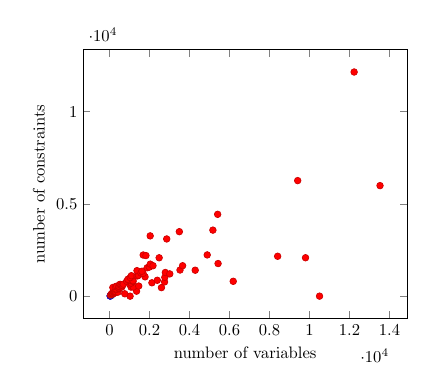
\begin{tikzpicture}[scale=0.6]
\begin{axis}[scatter, point meta=\thisrow{time}, only marks, , xlabel=number of variables,ylabel=number of constraints]

\addplot table[x=x,y=y]  { 
 x y time
 33 34 0.05 
 33 34 0.0 
 42 60 1.0 
 49 71 2880.0 
 98 68 189.0 
 80 107 2880.0 
 84 116 2591.0 
 104 151 2880.0 
 112 165 2880.0 
 143 164 2880.0 
 141 180 2880.0 
 1027 26 2880.0 
 181 159 2880.0 
 163 185 2880.0 
 226 197 2880.0 
 204 250 2880.0 
 283 206 2880.0 
 204 295 2880.0 
 263 264 2880.0 
 309 242 2880.0 
 250 305 2880.0 
 164 495 2880.0 
 302 281 2880.0 
 423 246 2880.0 
 761 155 2880.0 
 316 381 2880.0 
 354 404 2880.0 
 303 545 2880.0 
 481 421 2880.0 
 359 565 2880.0 
 474 446 2880.0 
 458 469 2880.0 
 473 539 2880.0 
 468 566 2880.0 
 10501 27 2880.0 
 615 522 2880.0 
 501 648 2880.0 
 535 666 2880.0 
 588 622 2880.0 
 646 601 2880.0 
 1351 295 2880.0 
 689 673 2880.0 
 1076 516 2880.0 
 1185 520 2880.0 
 1001 682 2880.0 
 855 829 2880.0 
 1076 732 2880.0 
 947 881 2880.0 
 1459 573 2880.0 
 915 937 2880.0 
 1176 821 2880.0 
 1170 863 2880.0 
 1036 1030 2880.0 
 1093 1133 2880.0 
 2595 487 2880.0 
 1377 1117 2880.0 
 2119 749 2880.0 
 1444 1147 2880.0 
 1776 1071 2880.0 
 1372 1405 2880.0 
 1572 1276 2880.0 
 1678 1255 2880.0 
 2388 885 2880.0 
 2751 795 2880.0 
 1621 1373 2880.0 
 2764 1045 2880.0 
 1881 1561 2880.0 
 1989 1598 2880.0 
 2037 1756 2880.0 
 2173 1673 2880.0 
 2790 1306 2880.0 
 3012 1231 2880.0 
 1682 2250 2880.0 
 1819 2221 2880.0 
 3524 1439 2880.0 
 6185 829 2880.0 
 2481 2101 2880.0 
 3653 1671 2880.0 
 4284 1429 2880.0 
 2032 3285 2880.0 
 2858 3119 2880.0 
 5428 1789 2880.0 
 4884 2256 2880.0 
 3490 3512 2880.0 
 8406 2183 2880.0 
 5168 3596 2880.0 
 9800 2103 2880.0 
 5406 4450 2880.0 
 9409 6273 2880.0 
 13526 6001 2880.0 
 12231 12143 2880.0 
};

\end{axis}
\end{tikzpicture}

\\
\tikz{\node (a) at (0.0,2.5) {\textsc{TheoMod}};\node (a) at (0.0,0) {};} & 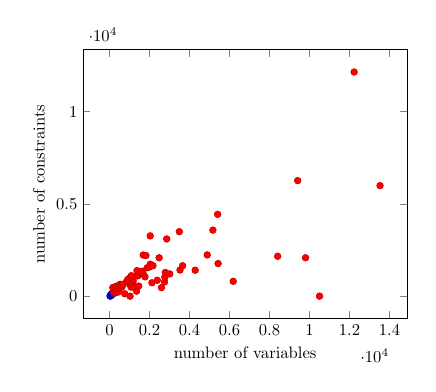
\begin{tikzpicture}[scale=0.6]
\begin{axis}[scatter, point meta=\thisrow{time}, only marks, , xlabel=number of variables,ylabel=number of constraints]

\addplot table[x=x,y=y]  { 
 x y time
 33 34 0.05 
 33 34 0.0 
 42 60 0.0 
 49 71 0.0 
 98 68 0.0 
 80 107 0.0 
 84 116 0.0 
 104 151 1.0 
 112 165 2.0 
 143 164 3.0 
 141 180 5.0 
 1027 26 2880.0 
 181 159 7.0 
 163 185 7.0 
 226 197 2880.0 
 204 250 2880.0 
 283 206 2880.0 
 204 295 2880.0 
 263 264 2880.0 
 309 242 2880.0 
 250 305 2880.0 
 164 495 2880.0 
 302 281 2880.0 
 423 246 2880.0 
 761 155 2880.0 
 316 381 2880.0 
 354 404 2880.0 
 303 545 2880.0 
 481 421 2880.0 
 359 565 2880.0 
 474 446 2880.0 
 458 469 2880.0 
 473 539 2880.0 
 468 566 2880.0 
 10501 27 2880.0 
 615 522 2880.0 
 501 648 2880.0 
 535 666 2880.0 
 588 622 2880.0 
 646 601 2880.0 
 1351 295 2880.0 
 689 673 2880.0 
 1076 516 2880.0 
 1185 520 2880.0 
 1001 682 2880.0 
 855 829 2880.0 
 1076 732 2880.0 
 947 881 2880.0 
 1459 573 2880.0 
 915 937 2880.0 
 1176 821 2880.0 
 1170 863 2880.0 
 1036 1030 2880.0 
 1093 1133 2880.0 
 2595 487 2880.0 
 1377 1117 2880.0 
 2119 749 2880.0 
 1444 1147 2880.0 
 1776 1071 2880.0 
 1372 1405 2880.0 
 1572 1276 2880.0 
 1678 1255 2880.0 
 2388 885 2880.0 
 2751 795 2880.0 
 1621 1373 2880.0 
 2764 1045 2880.0 
 1881 1561 2880.0 
 1989 1598 2880.0 
 2037 1756 2880.0 
 2173 1673 2880.0 
 2790 1306 2880.0 
 3012 1231 2880.0 
 1682 2250 2880.0 
 1819 2221 2880.0 
 3524 1439 2880.0 
 6185 829 2880.0 
 2481 2101 2880.0 
 3653 1671 2880.0 
 4284 1429 2880.0 
 2032 3285 2880.0 
 2858 3119 2880.0 
 5428 1789 2880.0 
 4884 2256 2880.0 
 3490 3512 2880.0 
 8406 2183 2880.0 
 5168 3596 2880.0 
 9800 2103 2880.0 
 5406 4450 2880.0 
 9409 6273 2880.0 
 13526 6001 2880.0 
 12231 12143 2880.0 
};

\end{axis}
\end{tikzpicture}

 & 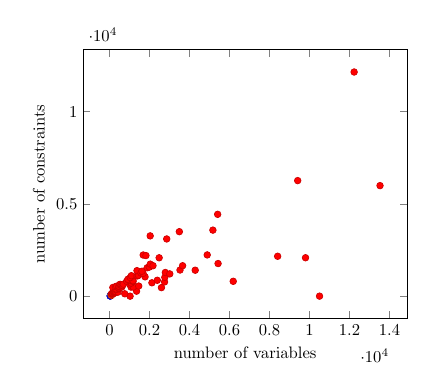
\begin{tikzpicture}[scale=0.6]
\begin{axis}[scatter, point meta=\thisrow{time}, only marks, , xlabel=number of variables,ylabel=number of constraints]

\addplot table[x=x,y=y]  { 
 x y time
 33 34 0.05 
 33 34 5.0 
 42 60 52.0 
 49 71 74.5 
 98 68 2880.0 
 80 107 1212.0 
 84 116 2579.0 
 104 151 2880.0 
 112 165 2880.0 
 143 164 2880.0 
 141 180 2880.0 
 1027 26 2880.0 
 181 159 2880.0 
 163 185 2880.0 
 226 197 2880.0 
 204 250 2880.0 
 283 206 2880.0 
 204 295 2880.0 
 263 264 2880.0 
 309 242 2880.0 
 250 305 2880.0 
 164 495 2880.0 
 302 281 2880.0 
 423 246 2880.0 
 761 155 2880.0 
 316 381 2880.0 
 354 404 2880.0 
 303 545 2880.0 
 481 421 2880.0 
 359 565 2880.0 
 474 446 2880.0 
 458 469 2880.0 
 473 539 2880.0 
 468 566 2880.0 
 10501 27 2880.0 
 615 522 2880.0 
 501 648 2880.0 
 535 666 2880.0 
 588 622 2880.0 
 646 601 2880.0 
 1351 295 2880.0 
 689 673 2880.0 
 1076 516 2880.0 
 1185 520 2880.0 
 1001 682 2880.0 
 855 829 2880.0 
 1076 732 2880.0 
 947 881 2880.0 
 1459 573 2880.0 
 915 937 2880.0 
 1176 821 2880.0 
 1170 863 2880.0 
 1036 1030 2880.0 
 1093 1133 2880.0 
 2595 487 2880.0 
 1377 1117 2880.0 
 2119 749 2880.0 
 1444 1147 2880.0 
 1776 1071 2880.0 
 1372 1405 2880.0 
 1572 1276 2880.0 
 1678 1255 2880.0 
 2388 885 2880.0 
 2751 795 2880.0 
 1621 1373 2880.0 
 2764 1045 2880.0 
 1881 1561 2880.0 
 1989 1598 2880.0 
 2037 1756 2880.0 
 2173 1673 2880.0 
 2790 1306 2880.0 
 3012 1231 2880.0 
 1682 2250 2880.0 
 1819 2221 2880.0 
 3524 1439 2880.0 
 6185 829 2880.0 
 2481 2101 2880.0 
 3653 1671 2880.0 
 4284 1429 2880.0 
 2032 3285 2880.0 
 2858 3119 2880.0 
 5428 1789 2880.0 
 4884 2256 2880.0 
 3490 3512 2880.0 
 8406 2183 2880.0 
 5168 3596 2880.0 
 9800 2103 2880.0 
 5406 4450 2880.0 
 9409 6273 2880.0 
 13526 6001 2880.0 
 12231 12143 2880.0 
};

\end{axis}
\end{tikzpicture}

\\
\\\\
\multicolumn{3}{c}{\ref{storedcolorbar1}}\end{tabular}\end{figure}

\newpage

\begin{figure}\caption{\textsc{Non-Equiv + Permut} for Test of 93 small instances of netlib}
\vspace{0.5cm}\centering

\begin{tabular}{ccc} & gecode & coinbc\\\\\tikz{\node (a) at (0.0,2.5) {\textsc{QuadraMod}};\node (a) at (0.0,0) {};} & 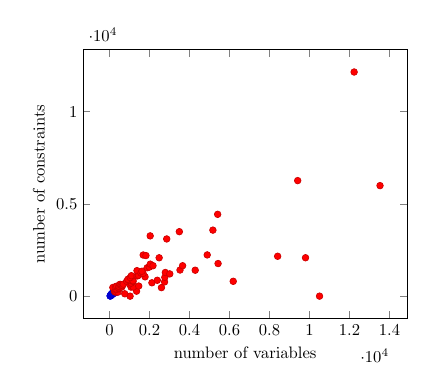
\begin{tikzpicture}[scale=0.6]
\begin{axis}[scatter, point meta=\thisrow{time}, only marks, colorbar, colorbar horizontal,colorbar style={ylabel={Time (min)}, ylabel style={rotate=270},}, colorbar to name={storedcolorbar2},, xlabel=number of variables,ylabel=number of constraints]

\addplot table[x=x,y=y]  { 
 x y time
 33 34 0.05 
 33 34 0.0 
 42 60 0.0 
 49 71 0.0 
 98 68 0.0 
 80 107 0.0 
 84 116 0.0 
 104 151 3.0 
 112 165 2.0 
 143 164 2.0 
 141 180 2.0 
 1027 26 2880.0 
 181 159 4.0 
 163 185 2.0 
 226 197 11.0 
 204 250 8.0 
 283 206 10.0 
 204 295 58.0 
 263 264 2880.0 
 309 242 2880.0 
 250 305 2880.0 
 164 495 2880.0 
 302 281 2880.0 
 423 246 2880.0 
 761 155 2880.0 
 316 381 2880.0 
 354 404 2880.0 
 303 545 2880.0 
 481 421 2880.0 
 359 565 2880.0 
 474 446 2880.0 
 458 469 2880.0 
 473 539 2880.0 
 468 566 2880.0 
 10501 27 2880.0 
 615 522 2880.0 
 501 648 2880.0 
 535 666 2880.0 
 588 622 2880.0 
 646 601 2880.0 
 1351 295 2880.0 
 689 673 2880.0 
 1076 516 2880.0 
 1185 520 2880.0 
 1001 682 2880.0 
 855 829 2880.0 
 1076 732 2880.0 
 947 881 2880.0 
 1459 573 2880.0 
 915 937 2880.0 
 1176 821 2880.0 
 1170 863 2880.0 
 1036 1030 2880.0 
 1093 1133 2880.0 
 2595 487 2880.0 
 1377 1117 2880.0 
 2119 749 2880.0 
 1444 1147 2880.0 
 1776 1071 2880.0 
 1372 1405 2880.0 
 1572 1276 2880.0 
 1678 1255 2880.0 
 2388 885 2880.0 
 2751 795 2880.0 
 1621 1373 2880.0 
 2764 1045 2880.0 
 1881 1561 2880.0 
 1989 1598 2880.0 
 2037 1756 2880.0 
 2173 1673 2880.0 
 2790 1306 2880.0 
 3012 1231 2880.0 
 1682 2250 2880.0 
 1819 2221 2880.0 
 3524 1439 2880.0 
 6185 829 2880.0 
 2481 2101 2880.0 
 3653 1671 2880.0 
 4284 1429 2880.0 
 2032 3285 2880.0 
 2858 3119 2880.0 
 5428 1789 2880.0 
 4884 2256 2880.0 
 3490 3512 2880.0 
 8406 2183 2880.0 
 5168 3596 2880.0 
 9800 2103 2880.0 
 5406 4450 2880.0 
 9409 6273 2880.0 
 13526 6001 2880.0 
 12231 12143 2880.0 
};

\end{axis}
\end{tikzpicture}

 & 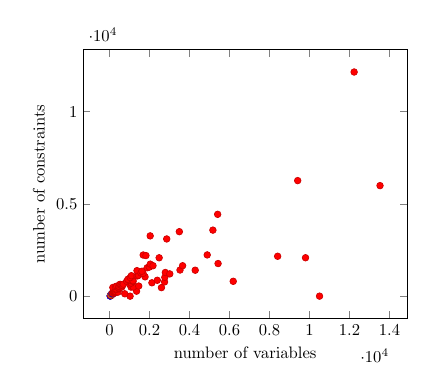
\begin{tikzpicture}[scale=0.6]
\begin{axis}[scatter, point meta=\thisrow{time}, only marks, , xlabel=number of variables,ylabel=number of constraints]

\addplot table[x=x,y=y]  { 
 x y time
 33 34 0.05 
 33 34 0.0 
 42 60 0.0 
 49 71 2880.0 
 98 68 2880.0 
 80 107 610.0 
 84 116 1872.0 
 104 151 2880.0 
 112 165 227.0 
 143 164 34.0 
 141 180 2880.0 
 1027 26 2880.0 
 181 159 11.0 
 163 185 2880.0 
 226 197 2880.0 
 204 250 2880.0 
 283 206 2880.0 
 204 295 2880.0 
 263 264 2880.0 
 309 242 2880.0 
 250 305 2880.0 
 164 495 2880.0 
 302 281 2880.0 
 423 246 2880.0 
 761 155 2880.0 
 316 381 2880.0 
 354 404 2880.0 
 303 545 2880.0 
 481 421 2880.0 
 359 565 2880.0 
 474 446 2880.0 
 458 469 2880.0 
 473 539 2880.0 
 468 566 2880.0 
 10501 27 2880.0 
 615 522 2880.0 
 501 648 2880.0 
 535 666 2880.0 
 588 622 2880.0 
 646 601 2880.0 
 1351 295 2880.0 
 689 673 2880.0 
 1076 516 2880.0 
 1185 520 2880.0 
 1001 682 2880.0 
 855 829 2880.0 
 1076 732 2880.0 
 947 881 2880.0 
 1459 573 2880.0 
 915 937 2880.0 
 1176 821 2880.0 
 1170 863 2880.0 
 1036 1030 2880.0 
 1093 1133 2880.0 
 2595 487 2880.0 
 1377 1117 2880.0 
 2119 749 2880.0 
 1444 1147 2880.0 
 1776 1071 2880.0 
 1372 1405 2880.0 
 1572 1276 2880.0 
 1678 1255 2880.0 
 2388 885 2880.0 
 2751 795 2880.0 
 1621 1373 2880.0 
 2764 1045 2880.0 
 1881 1561 2880.0 
 1989 1598 2880.0 
 2037 1756 2880.0 
 2173 1673 2880.0 
 2790 1306 2880.0 
 3012 1231 2880.0 
 1682 2250 2880.0 
 1819 2221 2880.0 
 3524 1439 2880.0 
 6185 829 2880.0 
 2481 2101 2880.0 
 3653 1671 2880.0 
 4284 1429 2880.0 
 2032 3285 2880.0 
 2858 3119 2880.0 
 5428 1789 2880.0 
 4884 2256 2880.0 
 3490 3512 2880.0 
 8406 2183 2880.0 
 5168 3596 2880.0 
 9800 2103 2880.0 
 5406 4450 2880.0 
 9409 6273 2880.0 
 13526 6001 2880.0 
 12231 12143 2880.0 
};

\end{axis}
\end{tikzpicture}

\\
\tikz{\node (a) at (0.0,2.5) {\textsc{TheoMod}};\node (a) at (0.0,0) {};} & 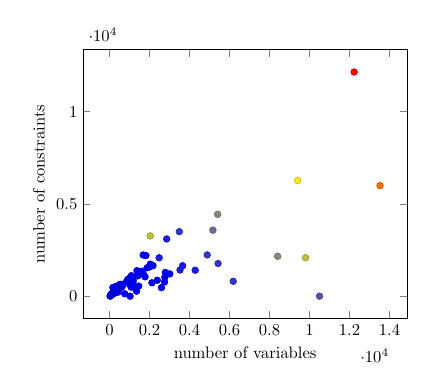
\begin{tikzpicture}[scale=0.6]
\begin{axis}[scatter, point meta=\thisrow{time}, only marks, , xlabel=number of variables,ylabel=number of constraints]

\addplot table[x=x,y=y]  { 
 x y time
 33 34 0.05 
 33 34 0.0 
 42 60 0.0 
 49 71 0.0 
 98 68 0.0 
 80 107 0.0 
 84 116 0.0 
 104 151 0.0 
 112 165 0.0 
 143 164 0.0 
 141 180 0.0 
 1027 26 0.0 
 181 159 0.0 
 163 185 0.0 
 226 197 0.0 
 204 250 0.0 
 283 206 0.0 
 204 295 0.0 
 263 264 0.0 
 309 242 0.0 
 250 305 0.0 
 164 495 0.0 
 302 281 0.0 
 423 246 0.0 
 761 155 0.0 
 316 381 0.0 
 354 404 0.0 
 303 545 0.0 
 481 421 0.0 
 359 565 0.0 
 474 446 0.0 
 458 469 0.0 
 473 539 0.0 
 468 566 0.0 
 10501 27 3.0 
 615 522 0.0 
 501 648 0.0 
 535 666 0.0 
 588 622 0.0 
 646 601 0.0 
 1351 295 0.0 
 689 673 0.0 
 1076 516 0.0 
 1185 520 0.0 
 1001 682 0.0 
 855 829 0.0 
 1076 732 0.0 
 947 881 0.0 
 1459 573 0.0 
 915 937 0.0 
 1176 821 0.0 
 1170 863 0.0 
 1036 1030 0.0 
 1093 1133 0.0 
 2595 487 0.0 
 1377 1117 0.0 
 2119 749 0.0 
 1444 1147 0.0 
 1776 1071 0.0 
 1372 1405 0.0 
 1572 1276 0.0 
 1678 1255 0.0 
 2388 885 0.0 
 2751 795 0.0 
 1621 1373 0.0 
 2764 1045 0.0 
 1881 1561 0.0 
 1989 1598 0.0 
 2037 1756 0.0 
 2173 1673 0.0 
 2790 1306 0.0 
 3012 1231 0.0 
 1682 2250 0.0 
 1819 2221 0.0 
 3524 1439 1.0 
 6185 829 2.0 
 2481 2101 1.0 
 3653 1671 1.0 
 4284 1429 1.0 
 2032 3285 7.0 
 2858 3119 1.0 
 5428 1789 2.0 
 4884 2256 2.0 
 3490 3512 2.0 
 8406 2183 5.0 
 5168 3596 4.0 
 9800 2103 7.0 
 5406 4450 5.0 
 9409 6273 11.0 
 13526 6001 20.0 
 12231 12143 28.0 
};

\end{axis}
\end{tikzpicture}

 & 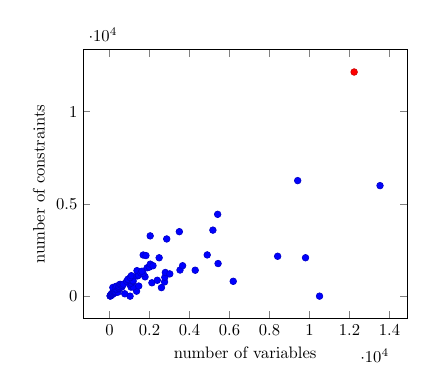
\begin{tikzpicture}[scale=0.6]
\begin{axis}[scatter, point meta=\thisrow{time}, only marks, , xlabel=number of variables,ylabel=number of constraints]

\addplot table[x=x,y=y]  { 
 x y time
 33 34 0.05 
 33 34 0.0 
 42 60 0.0 
 49 71 0.0 
 98 68 0.0 
 80 107 0.0 
 84 116 0.0 
 104 151 0.0 
 112 165 0.0 
 143 164 0.0 
 141 180 0.0 
 1027 26 0.0 
 181 159 0.0 
 163 185 0.0 
 226 197 0.0 
 204 250 0.0 
 283 206 0.0 
 204 295 0.0 
 263 264 0.0 
 309 242 0.0 
 250 305 0.0 
 164 495 0.0 
 302 281 0.0 
 423 246 0.0 
 761 155 0.0 
 316 381 0.0 
 354 404 0.0 
 303 545 0.0 
 481 421 0.0 
 359 565 0.0 
 474 446 0.0 
 458 469 0.0 
 473 539 0.0 
 468 566 0.0 
 10501 27 2.0 
 615 522 0.0 
 501 648 0.0 
 535 666 0.0 
 588 622 0.0 
 646 601 0.0 
 1351 295 0.0 
 689 673 0.0 
 1076 516 0.0 
 1185 520 0.0 
 1001 682 0.0 
 855 829 0.0 
 1076 732 0.0 
 947 881 0.0 
 1459 573 0.0 
 915 937 0.0 
 1176 821 0.0 
 1170 863 0.0 
 1036 1030 0.0 
 1093 1133 0.0 
 2595 487 0.0 
 1377 1117 0.0 
 2119 749 0.0 
 1444 1147 0.0 
 1776 1071 0.0 
 1372 1405 0.0 
 1572 1276 0.0 
 1678 1255 0.0 
 2388 885 0.0 
 2751 795 0.0 
 1621 1373 0.0 
 2764 1045 0.0 
 1881 1561 0.0 
 1989 1598 0.0 
 2037 1756 0.0 
 2173 1673 0.0 
 2790 1306 0.0 
 3012 1231 0.0 
 1682 2250 0.0 
 1819 2221 0.0 
 3524 1439 1.0 
 6185 829 1.0 
 2481 2101 0.0 
 3653 1671 1.0 
 4284 1429 1.0 
 2032 3285 12.0 
 2858 3119 1.0 
 5428 1789 1.0 
 4884 2256 1.0 
 3490 3512 2.0 
 8406 2183 4.0 
 5168 3596 3.0 
 9800 2103 4.0 
 5406 4450 4.0 
 9409 6273 11.0 
 13526 6001 17.0 
 12231 12143 2880.0 
};

\end{axis}
\end{tikzpicture}

\\
\\\\
\multicolumn{3}{c}{\ref{storedcolorbar2}}\end{tabular}\end{figure}

\newpage

\end{document}